\documentclass[a4paper, 12pt]{article}
\usepackage[a4paper,top=1.5cm, bottom=1.5cm, left=1cm, right=1cm]{geometry}
\usepackage{cmap}					
\usepackage{mathtext} 				
\usepackage[T2A]{fontenc}			
\usepackage[utf8]{inputenc}			
\usepackage[english,russian]{babel}
\usepackage{multirow}
\usepackage{graphicx}
\usepackage{wrapfig}
\usepackage{tabularx}
\usepackage{float}
\usepackage{longtable}
\usepackage{hyperref}
\hypersetup{colorlinks=true,urlcolor=blue}
\usepackage[rgb]{xcolor}
\usepackage{amsmath,amsfonts,amssymb,amsthm,mathtools} 
\usepackage{icomma} 
\usepackage{euscript}
\usepackage{mathrsfs}
\usepackage{enumerate}
\usepackage{caption}
\usepackage{enumerate}
\mathtoolsset{showonlyrefs=true}
\usepackage{graphicx}
\usepackage{caption}
\usepackage{subcaption}

\usepackage[europeanresistors, americaninductors]{circuitikz}
 \DeclareMathOperator{\sgn}{\mathop{sgn}}
\newcommand*{\hm}[1]{#1\nobreak\discretionary{}
	{\hbox{$\mathsurround=0pt #1$}}{}}


\title{\textbf{Определегие систематических и случайных погрешнойстей при измерении удельного сопротивления нихромовой проволоки (1.1.1)}}
\author{Павлушкин Вячеслав}
\date{Сентябрь 2021}




\begin{document}
	
	
	\maketitle
	      
	
	
	                     
	\section{Введение}
	
	\textbf{Цель работы:} измерить удельное сопротивление проволоки и вычислить систематические и случайные погрешности при использовании таких измерительных приборов, как линейка, штангенциркуль, микрометр, амперметр, вольтметр и мост постоянного тока.
	\bigskip\\
	\textbf{Оборудование:} линейка, штангенциркуль, микрометр, отрезок проволоки из нихрома, амперметр, вольтметр, источник ЭДС, мост постоянного тока, реостат, ключ.
	
	\section{Теоритические сведения}
		
		В данной работе измерять сопротивление $R_\text{пр}$ предлагается с помощью одной из схем представленных на рис. \ref{sexes}
			
		\begin{figure}[h]
			\centering
			\begin{subfigure}[t]{0.45\textwidth}
				\centering
				\begin{circuitikz}
					\draw (4.25, 0) to [pR, -., mirror, l=$R$, name=P] (3.1, 0)
					to [battery1, -., l=$\mathscr{E}$] (1, 0)
					to [rmeter, t=A] (1, -1.25)
					to [R, l=$R_A$] (1, -2.5)
					to (1, -4)
					to [rmeter, t=V] (2.5, -4)
					to [R, l=$R_V$] (4, -4)
					to (4.5, -4)
					to [nos] (4.5, 0)
					to (4.25, 0);
					\draw (3, 0) to [short] (2.8, 0) to [short] (2.8, 0.558) to (P.wiper);
					\draw (1, -3) to [R, l=$R_\text{пр}$] (4.5, -3) to (4.5, -3);
					\draw (1, -3) node[circ]{}
					(4.5, -3) node[circ]{};
			\end{circuitikz}
			\captionsetup{labelformat=empty}
			\caption{а)}
			\label{sex1}
		\end{subfigure}
		%
		\begin{subfigure}[t]{0.45\textwidth}
			\centering
			\begin{circuitikz}
				\draw (4.25, 0) to [pR, -., mirror, l=$R$, name=P] (3.1, 0)
				to [battery1, -., l=$\mathscr{E}$] (0, 0)
				to (0, -4)
				to [rmeter, t=V] (2.5, -4)
				to [R, l=$R_V$] (4, -4)
				to (4.5, -4)
				to [nos] (4.5, 0)
				to (4.25, 0);
				\draw (3, 0) to [short] (2.8, 0) to [short] (2.8, 0.558) to (P.wiper);
				\draw (0, -3) to [rmeter, t=A] (1.25, -3) to [R, l=$R_A$] (2.5, -3) to [R, l=$R_\text{пр}$] (4.5, -3) to (4.5, -3);
				\draw (0, -3) node[circ]{}
				(4.5, -3) node[circ]{};
			\end{circuitikz}
			\captionsetup{labelformat=empty}
			\caption{b)}
			\label{sex2}
		\end{subfigure}
	\caption{Схемы для измерения сопротивления}
	\label{sexes}
	\end{figure}
	
	Пусть $V$ и $I$ -- показания вольтметра и амперметра, при расчете сопротивления только этими данными: $R_\text{пр1} = V_\text{а}/I_\text{а}$ для схемы (\ref{sex1}) и  $R_\text{пр2} = V_\text{b}/I_\text{b}$ для схемы (\ref{sex2}) найденные сопротивления будут отличаться как друг от друга, так и от искомого $R_\text{пр}$ из-за внутренних сопротивлений приборов.
	
	\begin{center}{Учитывая сопротивления приборов получаем:}
	\end{center}
	
	\begin{minipage}{0.45\textwidth}
		\centering
		Для схемы (\ref{sex1})
		\begin{equation}\label{r1}
			R_\text{пр1} = \frac{V_a}{I_a} = R_\text{пр}\frac{R_V}{R_\text{пр} + R_V}
		\end{equation}
	\end{minipage}
	\begin{minipage}{0.45\textwidth}
		\centering
		Для схемы (\ref{sex2})
		\begin{equation}\label{r2}
			R_\text{пр2} = \frac{V_b}{I_b} = R_\text{пр} + R_A
		\end{equation}
	\end{minipage}
	
	\begin{center}
		Формулы (\ref{r1}) и (\ref{r2}) можно удобно преобразовать:
	
		\begin{minipage}{0.45\textwidth}
			\centering
			\begin{equation}\label{r3}
				R_\text{пр} = \frac{R_\text{пр1}}{1 - \left(\frac{R_\text{пр1}}{R_V} \right)} \approx R_\text{пр1}\left(1 + \frac{R_\text{пр1}}{R_V} \right)
			\end{equation}
		\end{minipage}
		\begin{minipage}{0.45\textwidth}
			\centering
			\begin{equation}\label{r4}
				R_\text{пр} = R_\text{пр2}\left(1-\frac{R_A}{R_\text{пр2}} \right)
			\end{equation}
		\end{minipage}
	\end{center}
		
	В разветленных цепях расчет поправок становится достаточно трудоемким и должен производиться заново при каждом переключении прибора. Таким образом получаем пример систематической ошибки, возникающей из-за упрощения расчетной формулы. Для схемы (\ref{sex1}) сопротивление $R_\text{пр}$ оказывается заниженным, а для схемы (\ref{sex2}) -- завышенным относительно рассчитанного.
	
	Более точным методом измерения сопротивлений является метод моста постоянного тока (мост Уитстона).
	
\section{Задание}
	\subsection{Знакомство со штангенциркулем и микрометром}
	
	\textbf{Штангенциркуль:} $ \sigma_\text{ш} = 0,05 \text{ мм}$\\
	\textbf{Микрометр:} $ \sigma_\text{м} = 0,01 \text{ мм}$
	
	
	\subsection{Измерение диаметра проволоки}
	\begin{table}[h]
		\begin{center}
			\begin{tabular}{|c|c|c|c|c|c|c|c|c|c|c|c|}
				\hline
				№ & 1 & 2 & 3 & 4 & 5 & 6 & 7 & 8 & 9 & 10 & ср. \\
				\hline
				$d_\text{ш}$, мм & 0,35 & 0,35& 0,35& 0,35& 0,35& 0,35& 0,35& 0,35& 0,35& 0,35& 0,35\\ 
				\hline
				$d_\text{м}$, мм & 0,34 & 0,36 & 0,36 & 0,35 & 0,36& 0,36& 0,36& 0,36& 0,36& 0,36& 0,357\\ 
				\hline
			\end{tabular}
		\end{center}
		\caption{Результаты измерения диаметра проволоки}
		\label{dtab}
	\end{table}
	
	При измерении штангенциркулем случайная погрешность отсутствует, а значит можно учитывать только системную погрешность: $d_\text{ш} = \left( 0,35 \pm 0,05 \right) \text{ мм}$.

	При измерении же микрометром нужно учитывать и системную и случайную погрешость:
	$$\sigma_\text{сист}=0,01\text{ мм}\;\;\;\;\;\; \sigma_\text{сл}=\frac{1}{N} \sqrt{\sum_{i=1}^{n}(d_i - \overline{d})^2}=\frac{1}{10} \sqrt{4,1\cdot 10^{-4}}\approx 2\cdot 10^{-3} \text{ мм}$$
	$$\sigma_{d_\text{м}} = \sqrt{\sigma_\text{сист}^2+\sigma_\text{сл}^2}\approx 0,01 \text{ мм}$$
	\noindent тогда $d_\text{м} = \left( 0,357 \pm 0,01 \right) \text{ мм}$.
	
	Площадь поперечного сечения проволоки можно вычислить зная диаметр, используя диаметр найденный с помощью микрометра мы уменьшим погрешность площади. Вычислим площадь и ее погрешность:
	
	\begin{equation}
		S_\text{пр} = \frac{\pi d_\text{м}^2}{4} = \frac{3,1415\cdot (0,357)^2}{4} \approx 0,1 \text{ мм}^2
	\end{equation}
	
	\begin{equation}
		\sigma_S = 2\frac{\sigma_{d_\text{м}}}{d_\text{м}}\cdot S = 2\frac{0,01}{0,357} \cdot 0,1 \approx 5,6\cdot 10^{-3} \text{ мм}^2
	\end{equation}

	С учетом погрешности получаем, что $S_\text{пр} = \left( 0,1 \pm 5,6 \cdot 10^{-3}\right) \text{ мм}^2$ т.е. площадь поперченого сечения определена с точностью 5,6\%
	
	\subsection{Характеристики измерительных приборов}
	\begin{longtable}[H]{|c|c|c|}
		\hline
		& Вольтметр & Миллиамперметр\\
		\hline
		Система & Магнитоэлектрическая & Цифровая \\
		Класс точности & 0,2 & --- \\
		Предел измерений $x_\text{П}$ & 0,6 В & 2 А -- 0,5 А\\
		Число делений шкалы $n$ & 150 & ---\\
		Цена делений $x_\text{П}/n$ & 4 мВ/дел & ---\\
		Чувствительность $n/x_\text{П}$ & 250 дел/В & --- \\
		Абсолютная погрешность $\Delta x_\text{М}$ & 2 мВ & 0,06 мА -- 0,6 мА\\
		Внутреннее сопротивление прибора & 4000 Ом & 1,2 Ом \\
		\hline
	\end{longtable}

	\subsection{Измерение поправок при измерении сопротивления}
	
	Поправки при измерении $R_\text{пр}$ это дополнительные коэффиценты на которые мы умножаем полученное сопротивление, для учета сопротивления измерительных приборов. Для схемы (\ref{sex1}) Эта поправка будет равняться $\frac{R_\text{пр1}}{R_V}\cdot 100\% = 0,125\%$, а для схемы (\ref{sex2}) $\frac{R_A}{R_\text{пр2}} \cdot 100\% = 3\%$.
	
	Чем меньше поправка тем лучше, следовательно для измерения сопротивления будем использовать схему (\ref{sex1}).
	
	\subsection{Снятие показаний вольтметра и амперметра, обработка полученных данных}
	
	Собираем схему и снимаем данные для разных длин проволоки: $l_1=(20,0 \pm 0,1)\text{ см}$; $l_2=(30,0 \pm 0,1) \text{, см}$; $ l_3=(50,0 \pm 0,1)\text{ см}$. Получаем:
	\begin{longtable}[H]{|c|c|c||c|c|c||c|c|c|}
		\hline
		\multicolumn{3}{|c||}{$l = 20 \text{ см}$} & \multicolumn{3}{c||}{$l = 30 \text{ см}$} & \multicolumn{3}{c|}{$l = 50 \text{ см}$}  \\
		\hline
		V, дел & V, мВ & I, мА & V, дел & V, мВ & I, мА & V, дел & V, мВ & I, мА \\
		\hline
		150 & 600 & 230,94 & 150 & 600 & 167,77 & 149 & 596 & 101,20 \\
		\hline
		138 & 552 & 211,53 & 134 & 536 & 150,26 & 141 & 564 & 95,58 \\
		\hline
		120 & 480 & 184,08 & 125 & 500 & 140,49 & 128 & 512 & 86,85 \\
		\hline
		104 & 416 & 158,45 & 109 & 436 & 122,52 & 121 & 484 & 81,9 \\
		\hline
		90 & 360 & 136,74 & 95 & 380 & 106,49 & 117 & 468 & 78,83 \\
		\hline
		81 & 324 & 123,42 & 85 & 340 & 95,18 & 107 & 428 & 72,29 \\
		\hline
		67 & 268 & 102,13 & 75 & 300 & 83,69 & 101 & 404 & 68,54 \\
		\hline
		62 & 248 & 91,73 & 66 & 264 & 73,94 & 94 & 376 & 63,48 \\
		\hline
		55 & 220 & 84,52 & 58 & 232 & 65,29 & 88 & 352 & 59,71 \\
		\hline
		44 & 176 & 66,9 & 51 & 204 & 57,32 & 82 & 328 & 55,51 \\
		\hline
		\caption{Снятая зависимость $V(I)$ для различных длин проволоки}
	\end{longtable}


	Построим графики по данным из таблицы: рис. \ref{graph}.
	\begin{figure}[h!]
		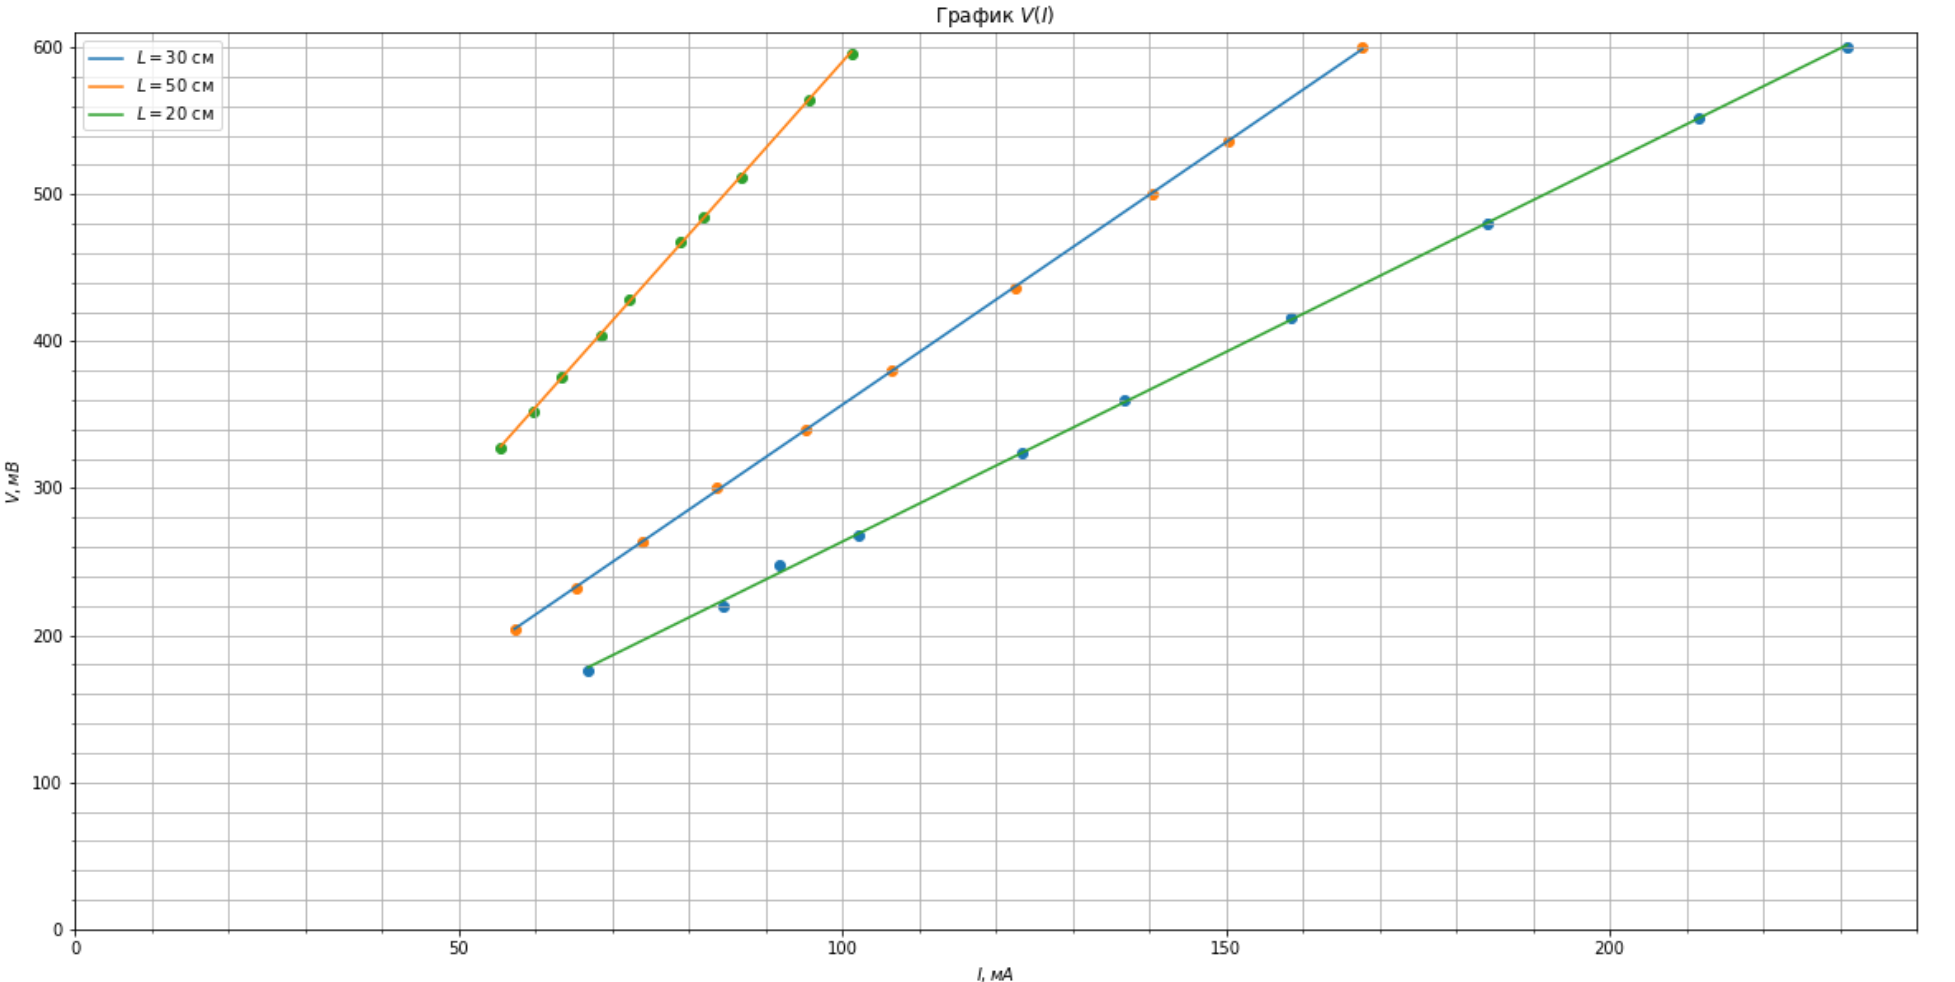
\includegraphics[scale = 0.55]{1.1.1_graph}
		\caption{Графики зависимости $V(I)$}
		\label{graph}
	\end{figure}
	
	Для каждой длины проволоки $l$ найдем  сопротивление и погрешности методом наименьших квадратов по формулам:
	
	\begin{equation}
		R_\text{ср} = \frac{\langle VI\rangle}{\langle I^2 \rangle}
	\end{equation}


	\begin{minipage}{0.45\textwidth}
		\centering
		\begin{equation}
			\sigma_{R_\text{ср}}^{\text{случ}} = \frac{1}{\sqrt{10}}\sqrt{\frac{\langle V^2 \rangle}{\langle I^2 \rangle} - R_\text{ср}^2}
		\end{equation}
	\end{minipage}
	\begin{minipage}{0.45\textwidth}
		\centering
		
		\begin{equation}
			\sigma_{R_\text{ср}}^{\text{сист}} = R_\text{ср}\sqrt{\left(\frac{\sigma_V}{V} \right)^2 + \left(\frac{\sigma_I}{I} \right)^2}
		\end{equation}
	\end{minipage}
	
	\begin{equation}
		\sigma_{R_\text{ср}} = \sqrt{\sigma_{\text{сист}}^2 + \sigma_{\text{случ}}^2}
	\end{equation}
	
	\noindent где $V$ и $I$ -- максимальные значения тока и напряжений, $\sigma_V = 2 \text{ мВ}$, а $\sigma_I = 0,6 \text{ мА}$. Рассчитываем сопротивление с учетом поправки для схемы (\ref{sex1}) и погрешности:
	
	\begin{longtable}[H]{|c||c||c|}
		\hline
		$l = 20 \text{ см}$ & $l = 30 \text{ см}$ & $l = 50 \text{ см}$ \\
		\hline
		$R_\text{ср} = 2,578 \text{ Ом}$ & $R_\text{ср} = 3,566 \text{ Ом}$ & $R_\text{ср} = 5,869 \text{ Ом}$ \\
		\hline
		$R_\text{пр} = 2,581 \text{ Ом}$ & $R_\text{пр} = 3,570 \text{ Ом}$ & $R_\text{пр} = 5,876 \text{ Ом}$\\
		\hline
		$\sigma_R^\text{случ} = 0,051\text{ Ом}$ & $\sigma_R^\text{случ} = 0,017\text{ Ом}$ & $\sigma_R^\text{случ} = 0,036\text{ Ом}$ \\
		\hline
		$\sigma_R^\text{сист} = 0,037 \text{ Ом}$ & $\sigma_R^\text{сист} = 0,051 \text{ Ом}$ & $\sigma_R^\text{сист} = 0,072 \text{ Ом}$ \\
		\hline
		$\sigma_{R_\text{ср}} = 0,063 \text{ Ом}$ & $\sigma_{R_\text{ср}} = 0,054 \text{ Ом}$ & $\sigma_{R_\text{ср}} = 0,081 \text{ Ом}$ \\
		\hline
		
		\caption{Экспериментально полученные сопротивления и погрешности}
		\label{R}
	\end{longtable}
	
	\subsection{Нахождение сопротивления с помощью моста}
	
	\begin{longtable}[H]{|c|c|c|c|}
		\hline
		l, см & 20 & 30 & 50 \\
		\hline
		$R_\text{пр} \text{, Ом}$ & 2,585 & 3,411 & 5,788 \\
		\hline
		
		\caption{Сопротивления, полученные с помощью моста}
		\label{most}
	\end{longtable}
	
	Сравниваем полученные экспериментальным путем результаты с полученными на мосте. Результаты измерений всех трех длин попадают в предел $\pm2\sigma_R$ из таб.\ref{R}.
	
	\subsection{Вычисление удельного сопроивления проволоки}
	
	Удельное сопротивление проволоки изготовленной из однородного материала и погрешность могут быть определены по формулам:
	
	\begin{minipage}{0.45\textwidth}
		\centering
		\begin{equation}
			\rho = R_\text{пр}\cdot\frac{S_\text{пр}}{l} = \frac{R_\text{пр}}{l} \cdot \frac{\pi d^2}{4}
		\end{equation}
	\end{minipage}
	\begin{minipage}{0.45\textwidth}
		\centering
		\begin{equation}
			\sigma_\rho = \rho\sqrt{\left(\frac{\sigma_R}{R}\right)^2 + \left( 2\frac{\sigma_d}{d} \right)^2 + \left( \frac{\sigma_l}{l}\right)^2}
		\end{equation}
		
	\end{minipage}
	
	\bigskip
	\noindent где $R_\text{пр}$ -- сопротивление измеряемого отрезка проволоки, $S_\text{пр}$ -- площадь поперечного сечения проволоки, $l$ -- его длина, а $d$ -- диаметр проволоки.
	
	Занесем полученные результаты в таблицу
	\begin{longtable}[H]{|c||c||c|}
		\hline
		$l \text{, см}$ & $\rho$, $ 10^{-6} \text{ Ом} \cdot \text{мм}^2 /\text{м}$ & $\sigma_\rho$, $ 10^{-6} \text{ Ом} \cdot \text{мм}^2 / \text{м}$\\
		\hline
		20 & 1,29 & 0,08\\
		\hline
		30 & 1,19 & 0,08\\
		\hline
		50 & 1,17 & 0,07\\
		\hline
		\caption{Удельные сопротивления участков проволоки различной длины}
	\end{longtable}

	Конечным значением удельного сопротивления лучше считать удельное сопротивления участка проволоки длиной 50 см, так как его сопротивление наибольшее, что означает наименьшую погрешность и наибольшую точность измерения. В таком случае: $\rho = \left( 1,17 \pm 0,07 \right) \cdot 10^{-6} \text{ Ом}\cdot \text{мм}^2/\text{м}$.
	
	\subsection{Вывод}
	
	Основной вклад в ошибку вносит погрешность при определении площади поперечного сечения, составляющая 5,6 \%, поэтому при измерении сопротивления достаточна точность 3 -- 4 \%. В нашем эксперименте она составила не более 2,5 \% и обуславливается главным образом погрешностью  аналогового вольтметра.
	
	При измерении диаметра проволоки точность микрометра оказалась слишком низкой для исследования проволоки на однородность по длине.
	
	Так же часть погрешности составляют соединительные провода, которые являются дополнительным сопротивлением.
	
	Допустимые значения удельного сопротивления нихрома: $\rho_\text{таб} = (0,97 - 1,14) \cdot 10^{-6} \text{ Ом}\cdot \text{мм}^2/\text{м}$ 	
	
	В случае с длиной проволоки 30 см и 50 см полученные значения попадают в табличные с учетом $\sigma_\rho$, однако при длине 20 см удельное сопротивление отличается на $2\sigma_\rho$.
	
	
	
	
	


	
	
	
	
	








\end{document}
